\documentclass[12pt]{beamer}
\usetheme{Boadilla}
\usepackage{booktabs}
\usepackage{enumitem}
\usepackage{tikz}
\newcommand{\E}{\mathbb{E}}
\usefonttheme{professionalfonts}
\usepackage{pgfplots}
\renewcommand{\arraystretch}{1.25}
\usetikzlibrary{trees}
\title[ECON2843]{Lecture 9}
\subtitle{Part 2 Probability and Distributions}
\date{}
\usepackage{amsmath,amssymb,mathtools,wasysym}
\begin{document}
	\begin{frame}
		\titlepage
	\end{frame}
	\begin{frame}
		\frametitle{Expected Value of a Uniform Distribution}
		
		\begin{align*}
			E(X) &= \int_{-\infty}^{\infty} x f(x) dx \\
			&= \int_a^b x \times \frac{1}{b-a} dx \\
			&= \frac{1}{b-a} \left[\frac{x^2}{2}\right]|_a^b \\
			&= \frac{b^2 - a^2}{2(b-a)} \\
			&= \frac{(b+a)(b-a)}{2(b-a)} \\
			&= \frac{a+b}{2}
		\end{align*}
		
	\end{frame}
\begin{frame}
	\frametitle{Variance}
	
		\begin{itemize}
		\item[\color{blue}$\blacktriangleright$] To calculate variance, we use the shortcut
		\begin{itemize}
			\item[\color{blue}$\blacktriangleright$] Mean $E(X) = \frac{a+b}{2}$
			\item[\color{blue}$\blacktriangleright$] $E(X^2)$:
			\begin{align*}
				E(X^2) &= \int_a^b x^2 \cdot \frac{1}{b-a} dx = \frac{a^2 + ab + b^2}{3}
			\end{align*}
			\item[\color{blue}$\blacktriangleright$] Apply the shortcut: $V(X) = E(X^2) - [E(X)]^2$
		\end{itemize}
		
		\item[\color{blue}$\blacktriangleright$] We have
			\[
			V(X) = \frac{(b-a)^2}{12}
			\]
	\end{itemize}
	
\end{frame}
\begin{frame}
	\frametitle{Example of Uniform Distribution: Patient Waiting Times}
	\begin{itemize}
		\item[\color{blue}$\blacktriangleright$] The length of time patients wait to see a doctor is uniformly distributed between 40 mins and 3 hrs.
		\item[\color{blue}$\blacktriangleright$] Let $X$ be the waiting time (in mins).
		\[f(x) = \frac{1}{140},\quad 40\le x\le180\]
	\end{itemize}
	\centering
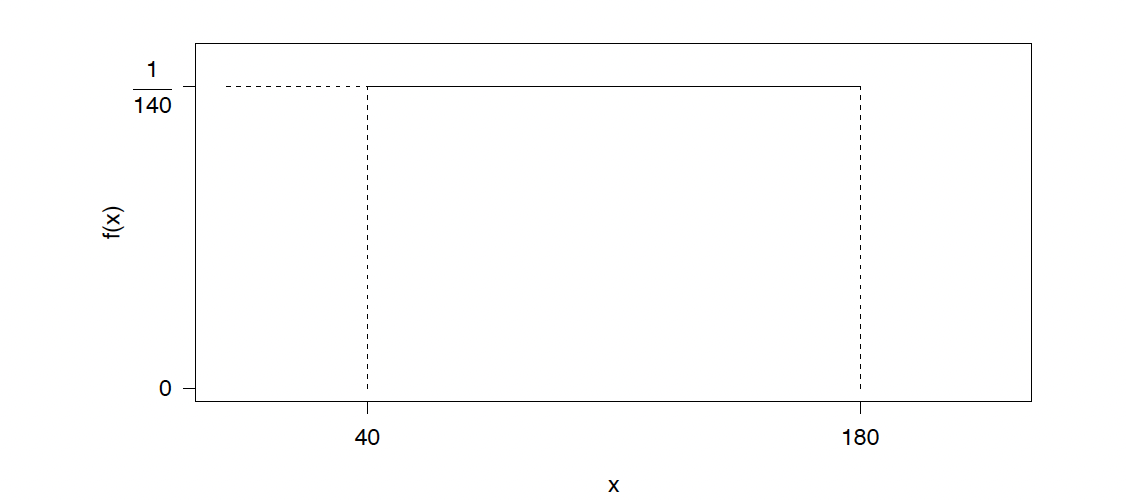
\includegraphics[width=8cm]{uniform.png}
\end{frame}
\begin{frame}
	\frametitle{Find the Probability of Waiting...}
	\begin{itemize}
		\item[\color{blue}$\blacktriangleright$] Between 1 and 2 hrs.
	\end{itemize}
	\centering
	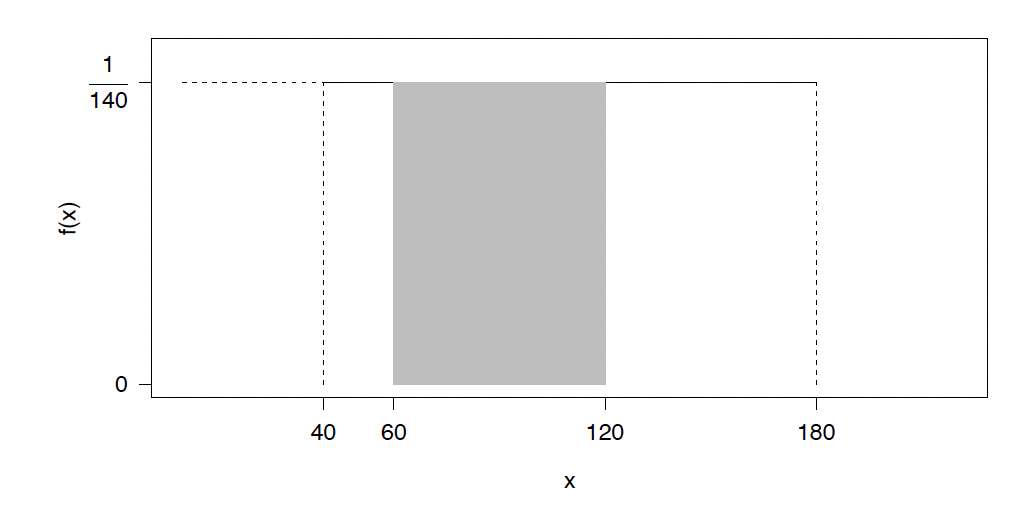
\includegraphics[width=10cm]{uniform2.png}
	\[P(60<X<120) = (120-60)\times\frac{1}{140}=\frac{3}{7}\]
\end{frame}
\begin{frame}
	\frametitle{Find the Probability of Waiting...}
	\begin{itemize}
		\item[\color{blue}$\blacktriangleright$] Between 1 and 2 hrs, given you waited over 90 min.
	\end{itemize}
	\centering
	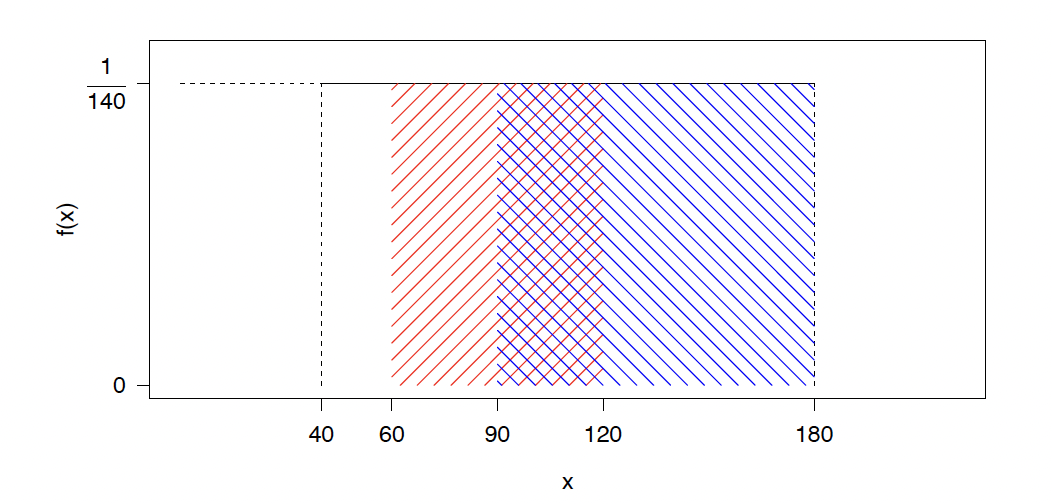
\includegraphics[width=10cm]{uniform3.png}
	\[P(\{60<X<120\}|\{X>90\})=\frac{P(90<X<120)}{P(X>90)}=\frac{\frac{3}{14}}{\frac{9}{14}}=\frac{1}{3}\]
\end{frame}
\begin{frame}
	\frametitle{Calculate the...}
	
	\begin{itemize}
	\item[\color{blue}$\blacktriangleright$] Mean and standard deviation of the waiting times.
	\end{itemize}
		\begin{align*}
			E(X) &= \frac{a + b}{2} = \frac{40 + 180}{2} = 110 \text{ min} \\[1em]
			V(X) &= \frac{(b - a)^2}{12} = \frac{(180 - 40)^2}{12} = 1633.3333 \text{ min}^2 \\[1em]
			SD(X) &= \sqrt{V(X)} = \sqrt{1633.333} = 40.4145 \text{ min}
		\end{align*}
	
\end{frame}
\begin{frame}
	\frametitle{Parachutist}
	
	\begin{itemize}
		\item[\color{blue}$\blacktriangleright$] A parachutist lands at a random point along the straight line between two markers, $A$ and $B$.
		\item[\color{blue}$\blacktriangleright$] Suppose the point at which they land is uniformly distributed between $A$ and $B$.
		\item[\color{blue}$\blacktriangleright$] Find the probability that their distance to $A$ is more than three times their distance to $B$.
	\end{itemize}
	
\end{frame}

\begin{frame}
	\frametitle{Probability Density Function}
	
	\begin{itemize}
		\item[\color{blue}$\blacktriangleright$] Let $X$ be the point at which the parachutist lands.
		\item[\color{blue}$\blacktriangleright$] Since we know $X\sim U(A,B)$, we know the PDF is
		$$f(x)=\frac{1}{B-A},\quad A\le x\le B$$
		\item[\color{blue}$\blacktriangleright$] We also know that $X$ lies between $A$ and $B$.
	\end{itemize}
	
\end{frame}
\begin{frame}
	\frametitle{Distance to Markers}
	
	\begin{itemize}
		\item[\color{blue}$\blacktriangleright$] Distance from $X$ to $A$ is $X - A$.
		
		\item[\color{blue}$\blacktriangleright$] Distance from $X$ to $B$ is $B - X$.
		
		\item[\color{blue}$\blacktriangleright$] We want:
		\begin{align*}
			P(X - A > 3(B - X)) &= P(4X > A + 3B) \\
			&= P\left(X > \frac{A + 3B}{4}\right)
		\end{align*}
		
		\item[\color{blue}$\blacktriangleright$] Let's sketch the PDF and shade the region of interest.
	\end{itemize}
	
	
\end{frame}

\begin{frame}
	\frametitle{Region of Interest}
	
\centering
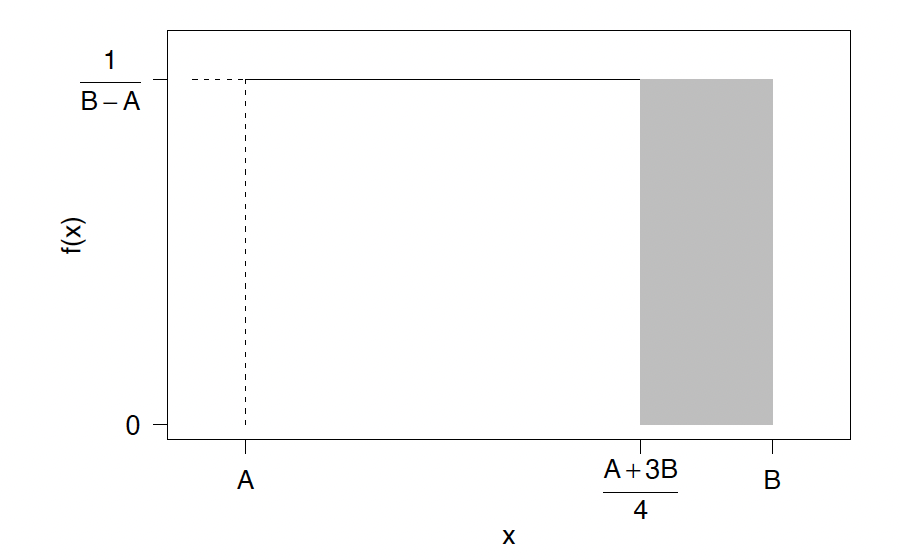
\includegraphics[width=10cm]{uniform4.png}
		$$P\left(X > \frac{A + 3B}{4}\right)=(B-(\frac{A+3B}{4}))\times\frac{1}{B-A}=\frac{1}{4}$$
	
	
\end{frame}

\begin{frame}
	\frametitle{Normal Distribution}
	
	\begin{itemize}
		\item[\color{blue}$\blacktriangleright$] A continuous random variable $X$ is said to have a 
		\textbf{normal distribution} with mean $\mu$ and variance $\sigma^2$ 
		if its PDF is given by the following function:
		
		\vspace{0.5em}
		\[
		f(x) = \frac{1}{\sigma\sqrt{2\pi}} e^{-\frac{(x-\mu)^2}{2\sigma^2}}, \quad -\infty < x < \infty
		\]
		\vspace{0.5em}
		
		\item[\color{blue}$\blacktriangleright$] We use the notation $X \sim N(\mu, \sigma^2)$.
		
		\item[\color{blue}$\blacktriangleright$] There are two {\sl parameters} that define the normal distribution, namely, $\mu$ and $\sigma^2$.
	\end{itemize}
	
\end{frame}

\begin{frame}
	\frametitle{Probability Density Function}
	
	\begin{itemize}
		\item[\color{blue}$\blacktriangleright$] Bell-shaped, symmetric about $\mu$, reaches highest point at $x=\mu$, tends to zero as $x\rightarrow\pm\infty$.
		

	\end{itemize}
	\centering
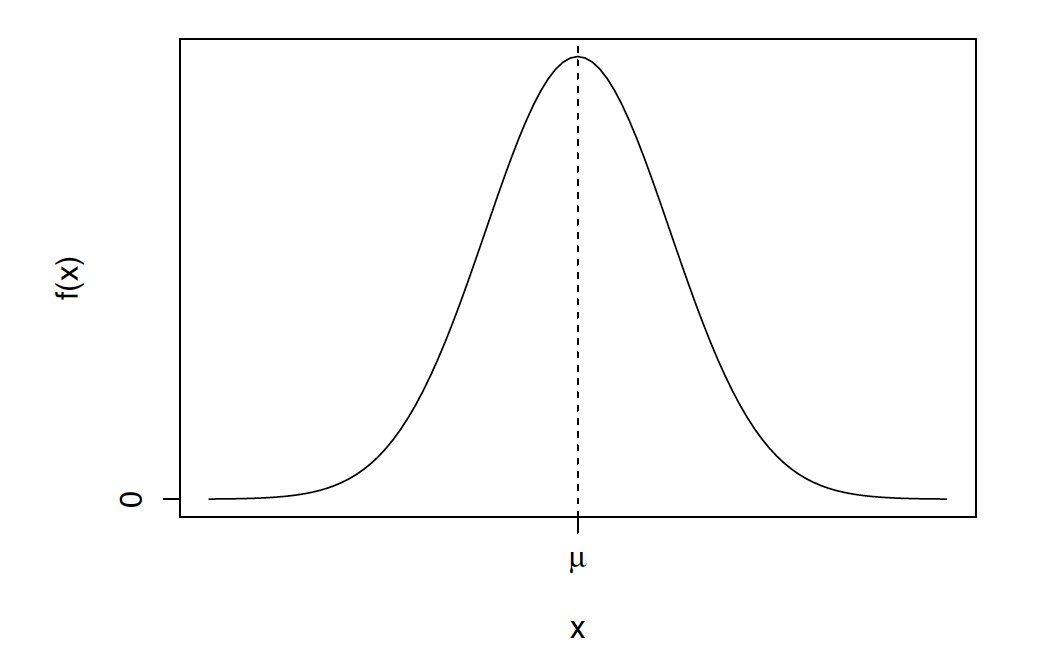
\includegraphics[width=10cm]{normal.png}
\end{frame}
\begin{frame}
	\frametitle{Properties}
	
	\begin{itemize}
		\item[\color{blue}$\blacktriangleright$] Total area under the curve equals 1.
		
		\item[\color{blue}$\blacktriangleright$] If we apply the formulae for $E(X)$ and $V(X)$ and 
		use some calculus, we can show that:
		
		\vspace{0.5em}
		\begin{align*}
			E(X) &= \mu \\
			V(X) &= \sigma^2
		\end{align*}
		\vspace{0.5em}
		
		\item[\color{blue}$\blacktriangleright$] Changing $\mu$ (different means) will shift the PDF 
		curve left and right along the $x$-axis.
		
		\item[\color{blue}$\blacktriangleright$] Changing $\sigma^2$ (different variances) will make the 
		PDF curve become more peaked or more flattened.
	\end{itemize}
	
\end{frame}
\begin{frame}
	\frametitle{Different Means, Same Variances}
	\centering
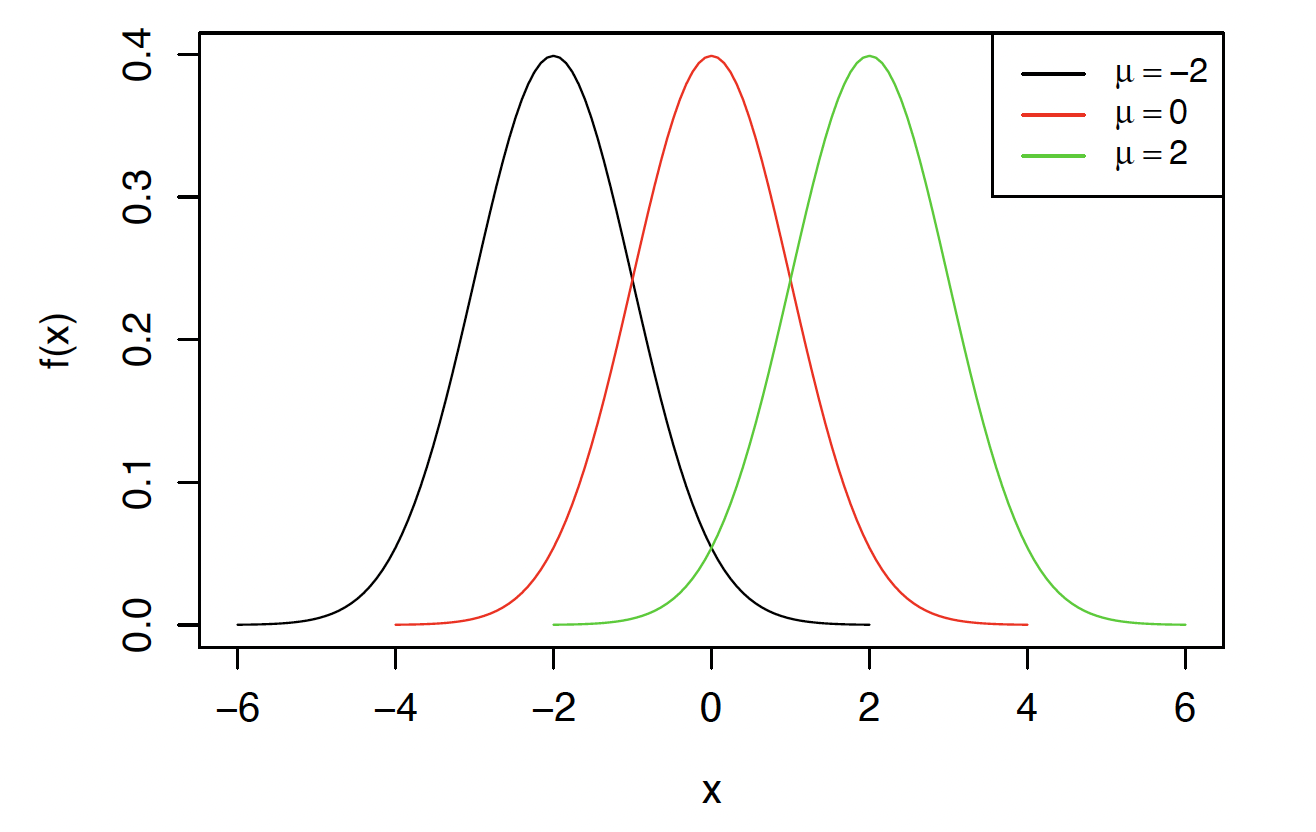
\includegraphics[width=12cm]{normal2.png}
\end{frame}
\begin{frame}
	\frametitle{Different Means, Same Variances}
	\centering
	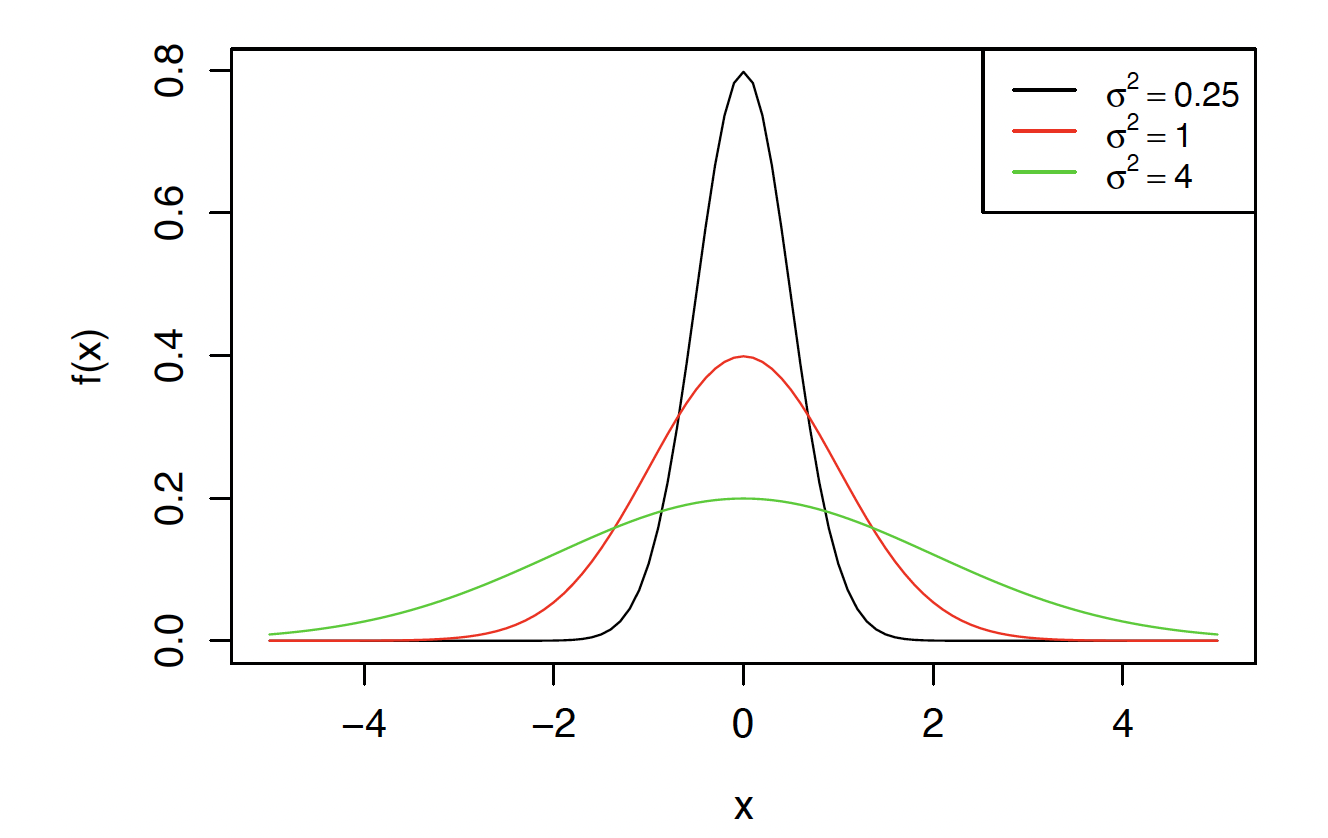
\includegraphics[width=12cm]{normal3.png}
\end{frame}
\begin{frame}
	\frametitle{Calculating Probabilities}
	\begin{itemize}
	\item[\color{blue}$\blacktriangleright$] How can we find $P(a < X < b)$, where $a$ and $b$ can be either positive, negative or $\pm\infty$?
	
	
\end{itemize}
	\centering
	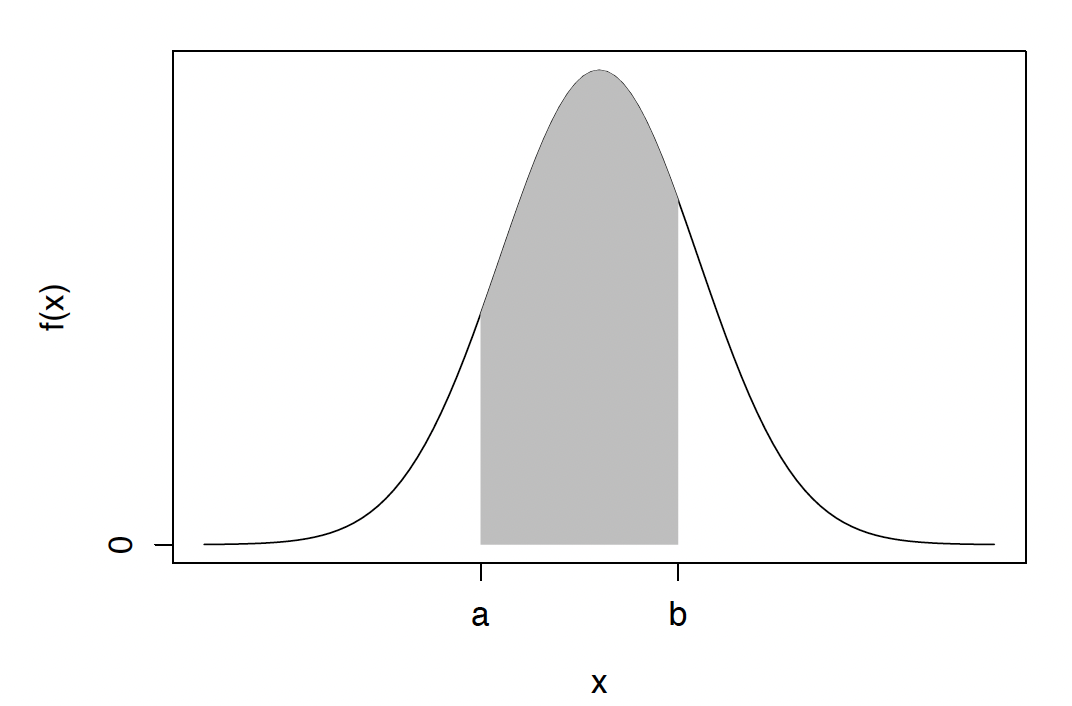
\includegraphics[width=10cm]{normal4.png}
\end{frame}

\begin{frame}
	\frametitle{Calculating Probabilities}
	
	\begin{itemize}
		\item[\color{blue}$\blacktriangleright$] We need to find the area under the PDF curve 
		between $a$ and $b$...
		
		\item[\color{blue}$\blacktriangleright$] That is, we need to perform the following 
		integration:
		
		\vspace{0.5em}
		\begin{align*}
			P(a < X < b) &= \int_a^b f(x)dx \\[1em]
			&= \int_a^b \frac{1}{\sigma\sqrt{2\pi}} e^{-\frac{(x-\mu)^2}{2\sigma^2}} dx
		\end{align*}
		\vspace{0.5em}
		
		\item[\color{blue}$\blacktriangleright$] Not easy to do!
	\end{itemize}
	
\end{frame}
\begin{frame}
	\frametitle{Statistical Tables}
	
	\begin{itemize}
		\item[\color{blue}$\blacktriangleright$] Statistical tables are available that list $P(X < a)$ for various values of $a$ for a normal distribution.
		 
		\item[\color{blue}$\blacktriangleright$] However, there are infinite number of normal distributions out there!
		
		\item[\color{blue}$\blacktriangleright$] Specifically, there is a different one for every different pair of values of $\mu$ and $\sigma^2$.
		\item[\color{blue}$\blacktriangleright$] How many tables do we need???
	\end{itemize}
	
\end{frame}

\begin{frame}
	\frametitle{Statistical Tables}
	
	\begin{itemize}
		\item[\color{blue}$\blacktriangleright$] It turns out we only need one statistical table for one specific normal distribution called the {\bf standard normal distribution}.
		
		\item[\color{blue}$\blacktriangleright$] The standard normal distribution is a normal distribution with $\mu=0$ and $\sigma^2=1$, i.e., $N(0,1)$.
		
		\item[\color{blue}$\blacktriangleright$] Any other normal distribution can be {\sl standardized} to become a $N(0,1)$ distribution.
	\end{itemize}
	
\end{frame}

\begin{frame}
	\frametitle{Standardizing a Normal Distribution}
	\centering
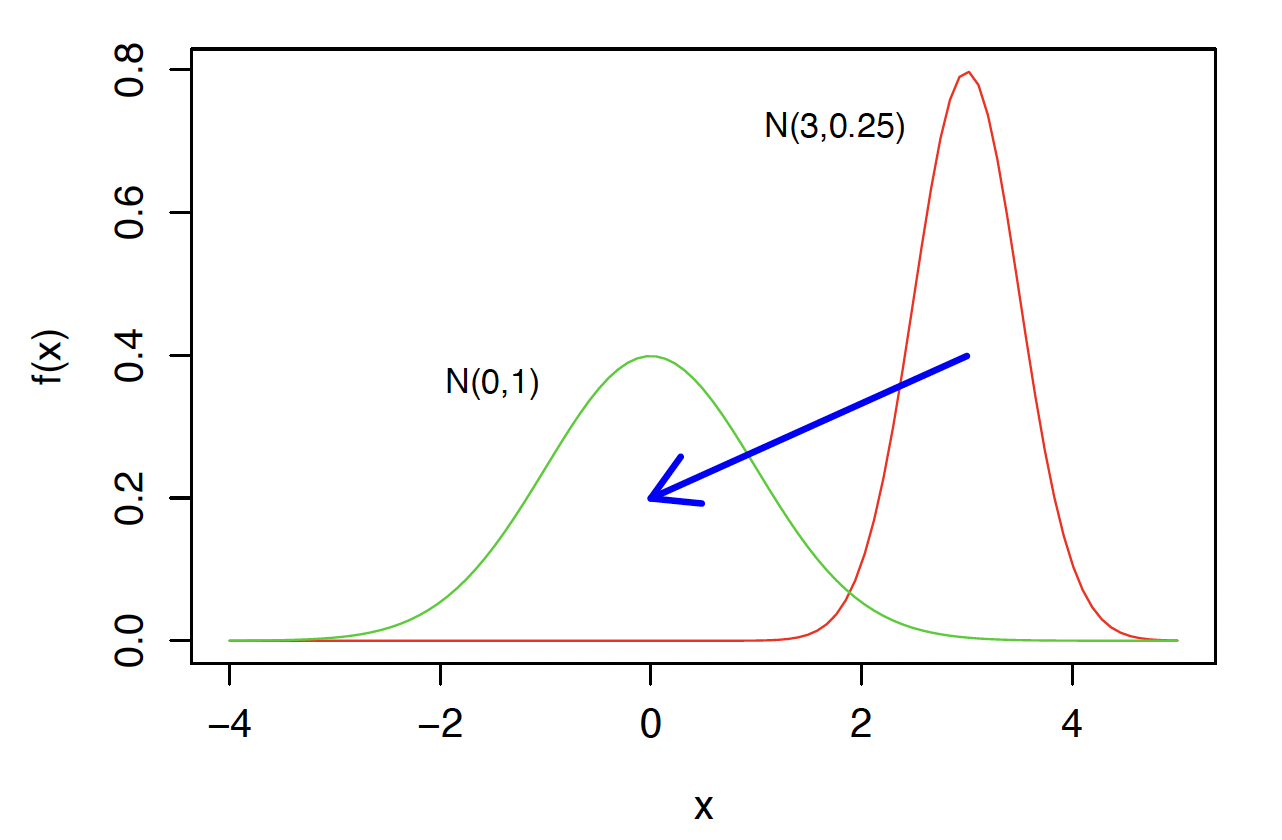
\includegraphics[width=10cm]{normal5.png}
\end{frame}

\begin{frame}
	\frametitle{Standardizing a Normal Distribution}
	
	\begin{itemize}
		\item[\color{blue}$\blacktriangleright$] If $X \sim N(\mu, \sigma^2)$, then the linear transformation
		\[
		Z = \frac{X - \mu}{\sigma} \sim N(0,1)
		\]
		standardizes $X$ to be a $N(0,1)$ random variable.
		
		\item[\color{blue}$\blacktriangleright$] The random variable $Z$ can be interpreted as the 
		number of standard deviations $X$ is away from $\mu$.
		
		\item[\color{blue}$\blacktriangleright$] The table of probabilities for a $Z \sim N(0,1)$ 
		distribution is called a $z$-table and it lists 
		probabilities of the form $P(Z < z)$ for various 
		values of $z$.
	\end{itemize}
	
	\end{frame}
	\begin{frame}
		\frametitle{$z$-Table}
	\centering
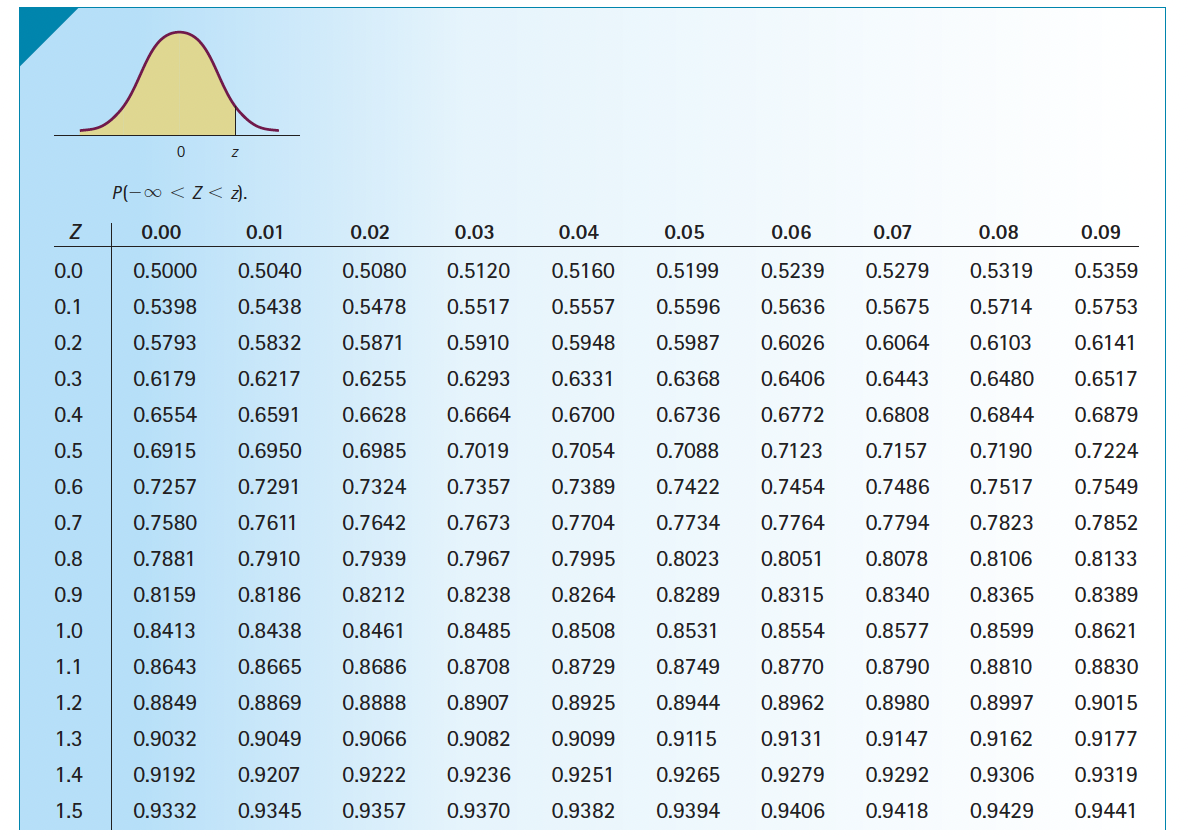
\includegraphics[width=10cm]{ztable.png}
	\end{frame}
		\begin{frame}
		\frametitle{Find $P(Z<0.63)$}
		\centering
		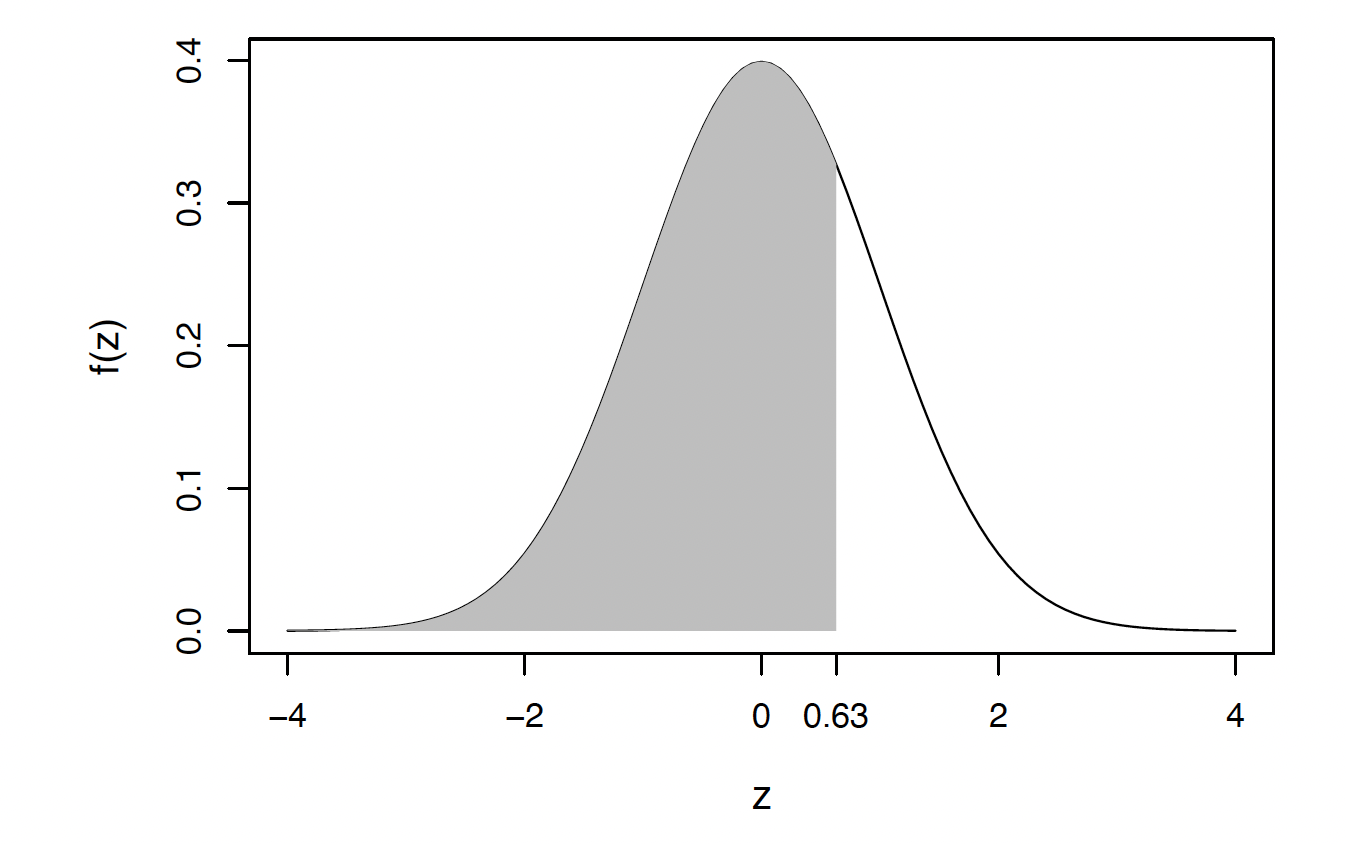
\includegraphics[width=12cm]{normal6.png}
	\end{frame}
		\begin{frame}
		\frametitle{Find $P(Z<0.63)$}
		\centering
		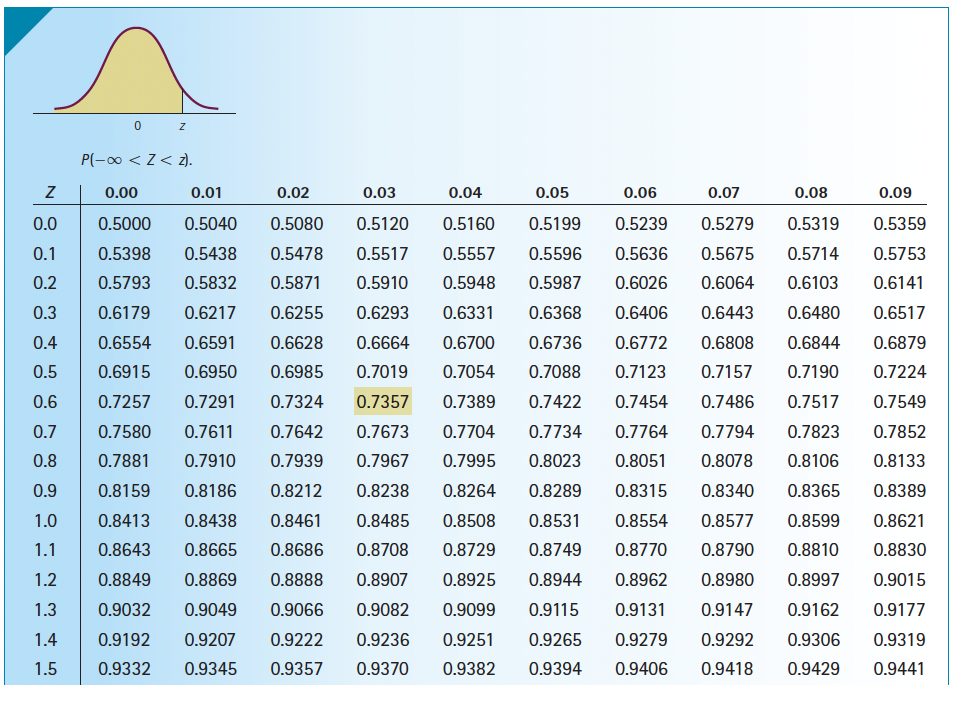
\includegraphics[width=10cm]{ztable2.png}
		$P(Z<0.63)=0.7357$
	\end{frame}
	\begin{frame}
		\frametitle{Find $P(Z>1.5)$}
		\centering
		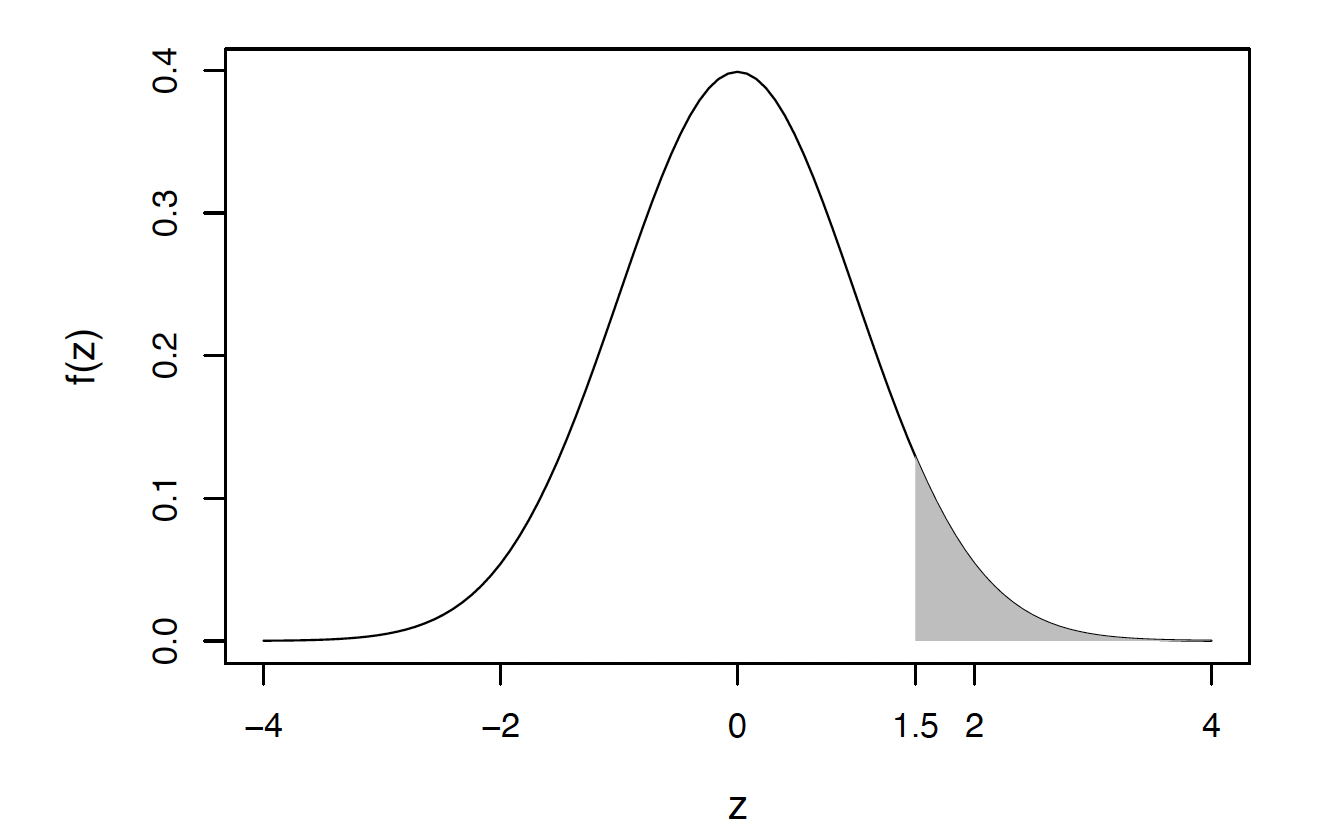
\includegraphics[width=12cm]{normal7.png}
	\end{frame}
\begin{frame}
	\frametitle{Find $P(Z>1.5)$}
	\centering
	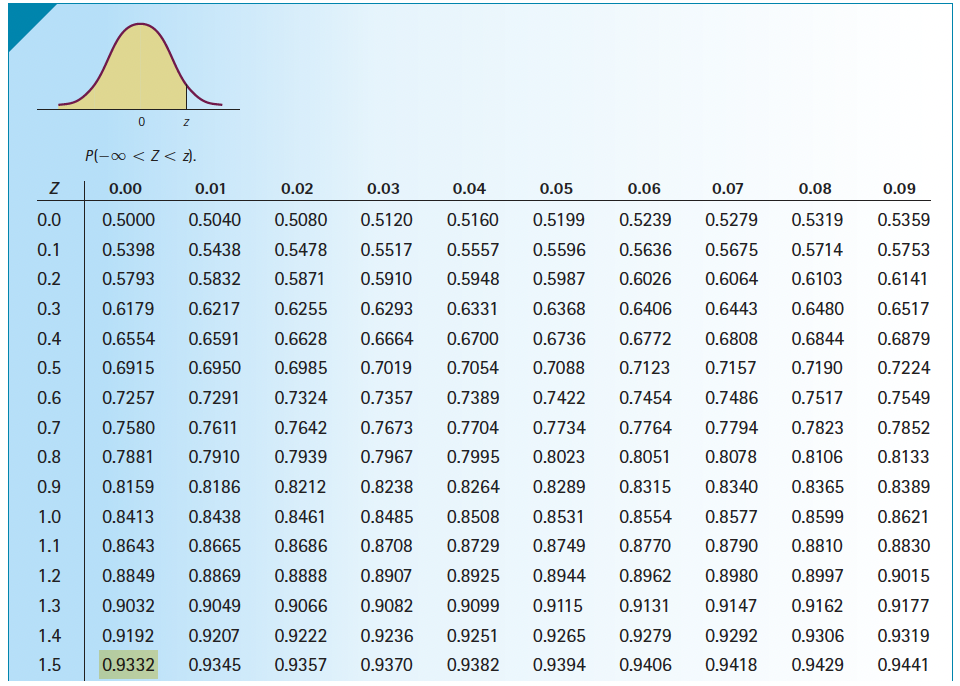
\includegraphics[width=10cm]{ztable3.png}
	$P(Z>1.5)=1-P(Z<1.5)=1-0.9332=0.0668$
\end{frame}
\begin{frame}
	\frametitle{Find $P(Z>1.5)$}
	\centering
	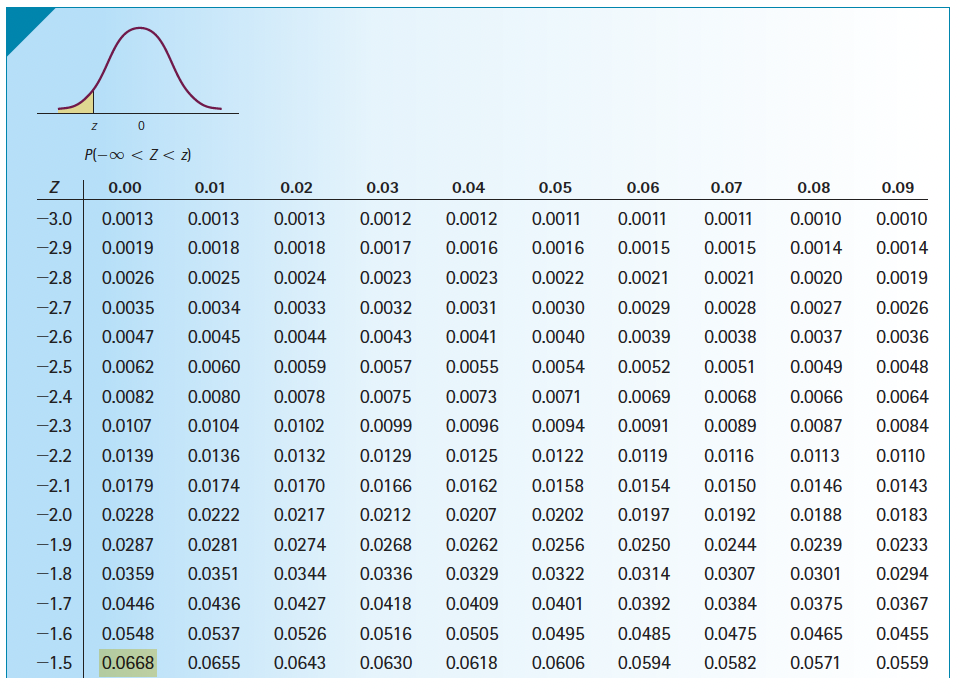
\includegraphics[width=10cm]{ztable4.png}
	$P(Z>1.5)=P(Z<-1.5)=0.0668$
\end{frame}
\begin{frame}
	\frametitle{Find $P(0.63<Z<1.5)$}
	\centering
	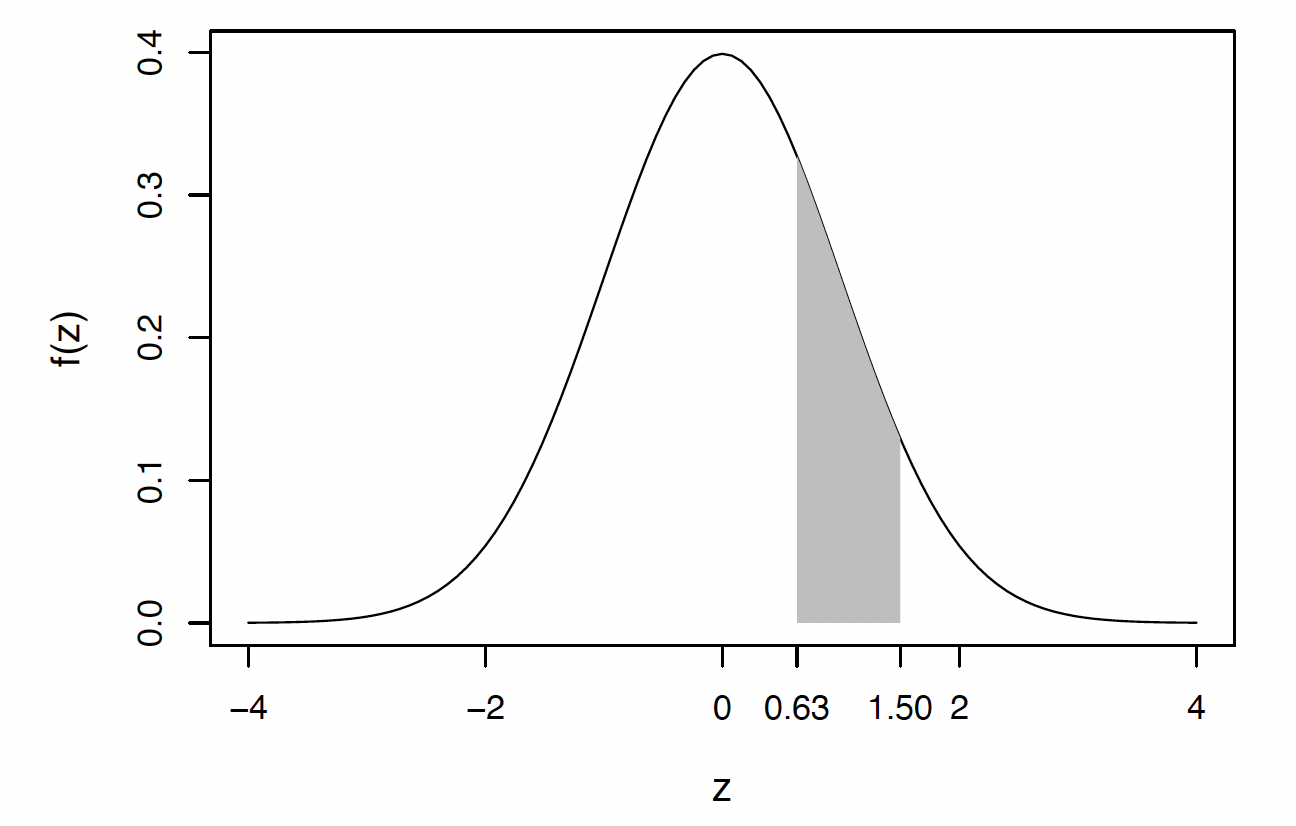
\includegraphics[width=12cm]{normal8.png}
\end{frame}
\begin{frame}
	\frametitle{Find $P(0.63<Z<1.5)$}
	\centering
	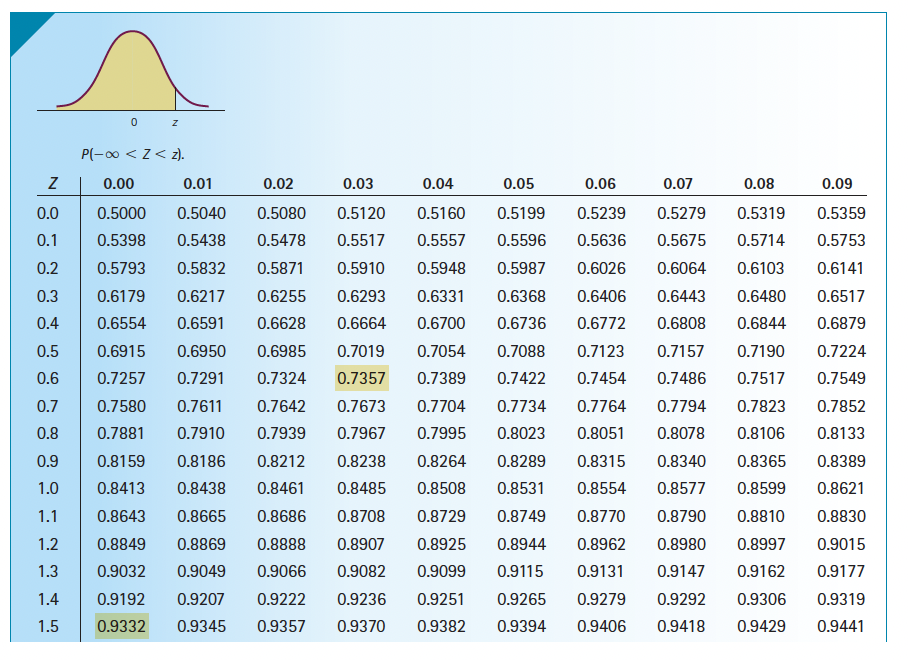
\includegraphics[width=9cm]{ztable5.png}
	\begin{align*}
		P(0.63<Z<1.5)&=P(Z<1.5)-P(Z<0.63)\\
		&=0.9332 =0.7357 = 0.1975
	\end{align*}
\end{frame}
\begin{frame}
	\frametitle{Example 1}
	
	\begin{itemize}
		\item[\color{blue}$\blacktriangleright$] The length of metallic strips produced by a machine 
		are normally distributed with a mean of 100cm and 
		a variance of 2.25cm$^2$.
		
		\item[\color{blue}$\blacktriangleright$] Only strips that are between 98cm and 103cm are 
		acceptable.
		
		\item[\color{blue}$\blacktriangleright$] What proportion of strips are acceptable?
		
		\item[\color{blue}$\blacktriangleright$] Let $X$ be the length of a metallic strip in cm.
		
		\item[\color{blue}$\blacktriangleright$] Then $X \sim N(\mu = 100, \sigma^2 = 2.25)$.
	\end{itemize}
	
	\end{frame}
	
	\begin{frame}
		\frametitle{Example 1}
\centering
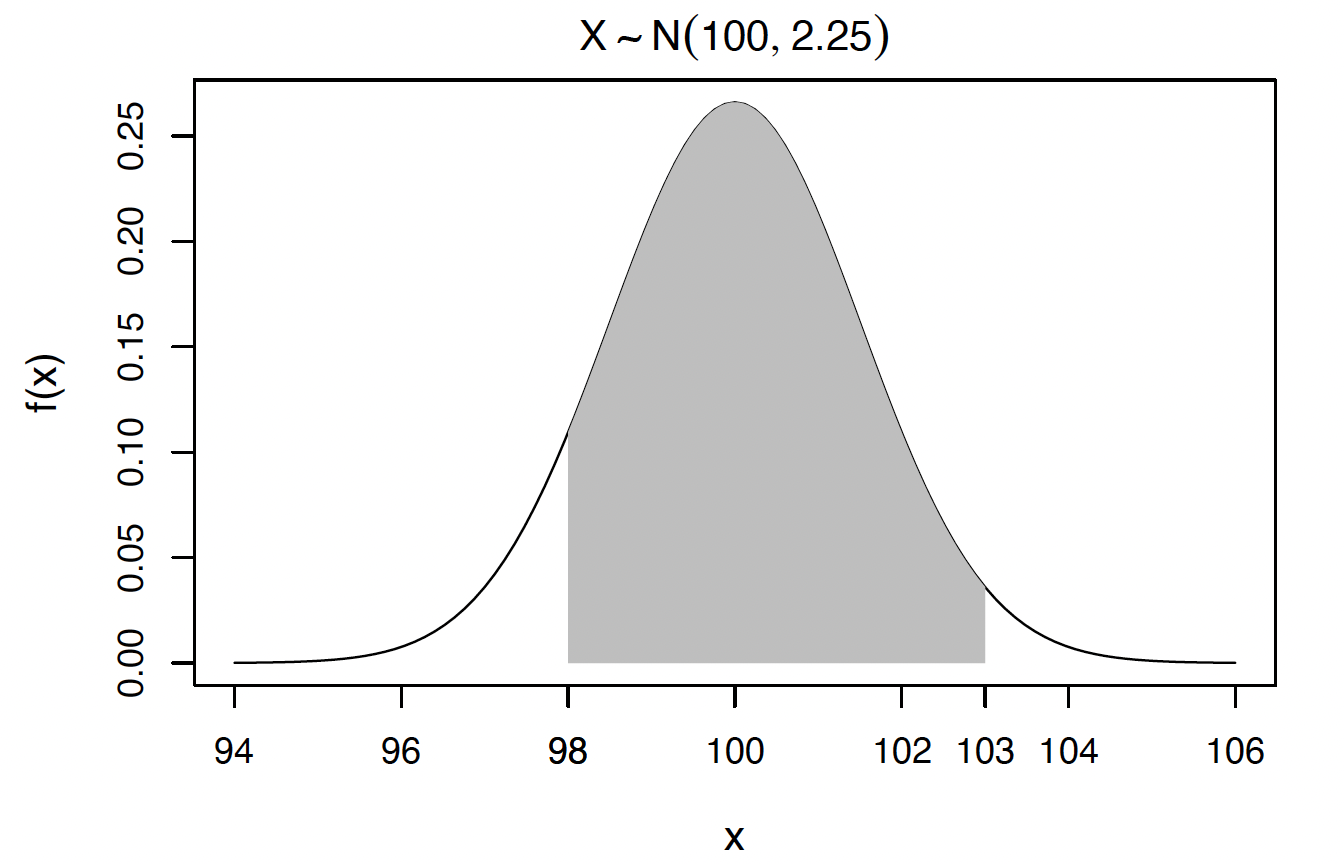
\includegraphics[width=12cm]{example1.png}
	\end{frame}

\begin{frame}
	\frametitle{Example 1}
	
	\begin{itemize}
		\item[\color{blue}$\blacktriangleright$] Firstly, we must standardize the $X$-distribution so 
		that we can find the values in the $Z$-distribution 
		that correspond to $X = 98$ and $X = 103$.
		
		\item[\color{blue}$\blacktriangleright$] Standardize $X = 98$:
		\[
		Z = \frac{X - \mu}{\sigma} = \frac{98 - 100}{\sqrt{2.25}} = -1.33
		\]
		
		\item[\color{blue}$\blacktriangleright$] Standardize $X = 103$:
		\[
		Z = \frac{X - \mu}{\sigma} = \frac{103 - 100}{\sqrt{2.25}} = 2
		\]
	\end{itemize}
	
	\end{frame}
	\begin{frame}
	\frametitle{Example 1: After Standardization}
	\centering
	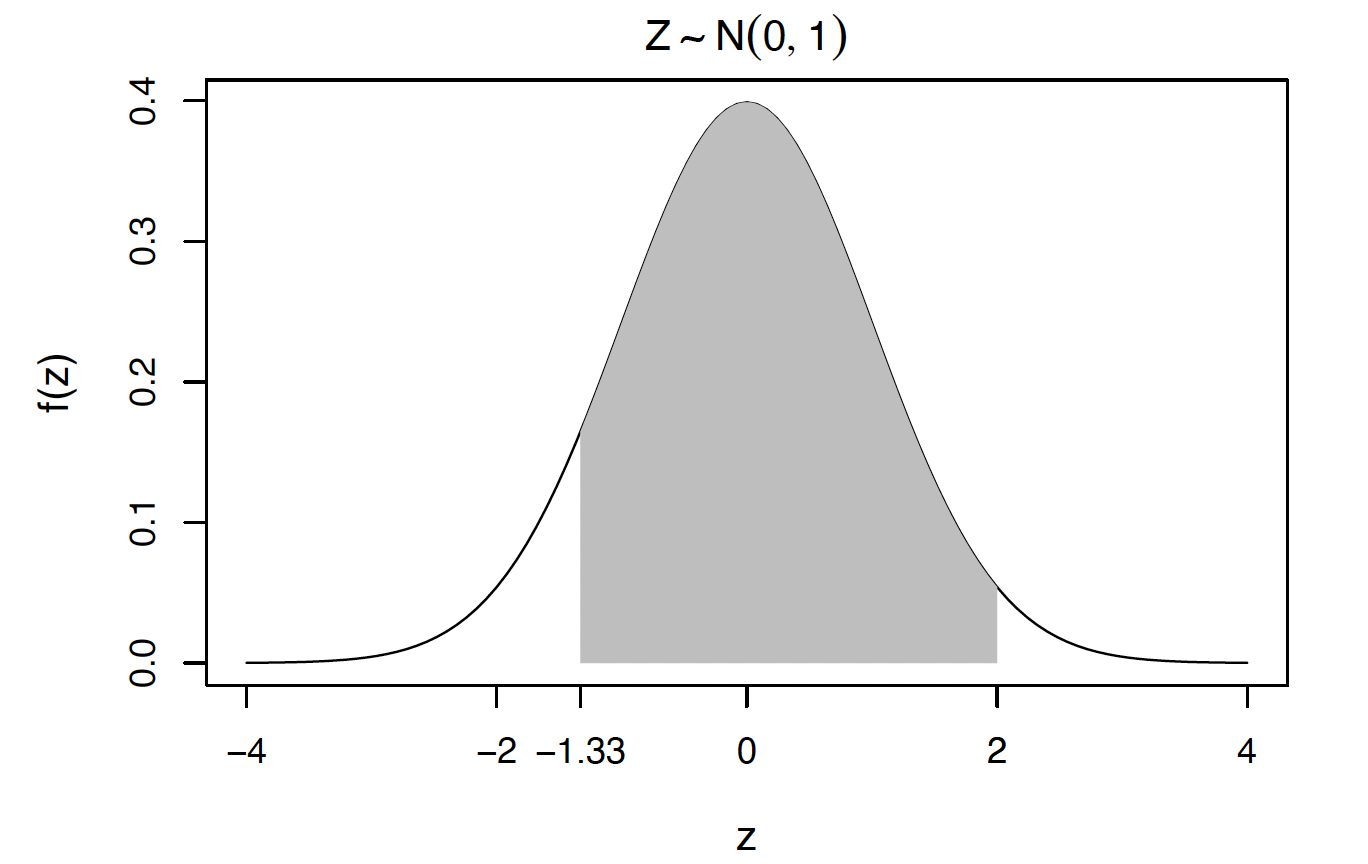
\includegraphics[width=12cm]{normal9.png}
\end{frame}
\begin{frame}
	\frametitle{Example 1}
	
	\begin{itemize}
		\item[\color{blue}$\blacktriangleright$] The area of the shaded region is equal to:
		\begin{align*}
			P(-1.33 < Z < 2) &= P(Z < 2) - P(Z < -1.33) \\
			&= 0.9772 - 0.0918 \\
			&= 0.8854
		\end{align*}
		
		\item[\color{blue}$\blacktriangleright$] So 88.54\% of metallic strips produced are 
		acceptable.
	\end{itemize}
	
\end{frame}

\begin{frame}
	\frametitle{Example 2}
	
	\begin{itemize}
		\item[\color{blue}$\blacktriangleright$] Salaries of workers in a factory are normally 
		distributed with mean \$48,000 and standard 
		deviation \$3,500.
		
		\item[\color{blue}$\blacktriangleright$] What is the minimum salary of the top 20\% of 
		workers?
		
		\item[\color{blue}$\blacktriangleright$] Let $X$ be the salary of a worker.
		
		\item[\color{blue}$\blacktriangleright$] Then $X \sim N(\mu = 48000, \sigma^2 = 3500^2)$.
		
		\item[\color{blue}$\blacktriangleright$] We want to find $a$ such that $P(X > a) = 0.2$.
	\end{itemize}
	
\end{frame}
	\begin{frame}
	\frametitle{Example 2}
	\centering
	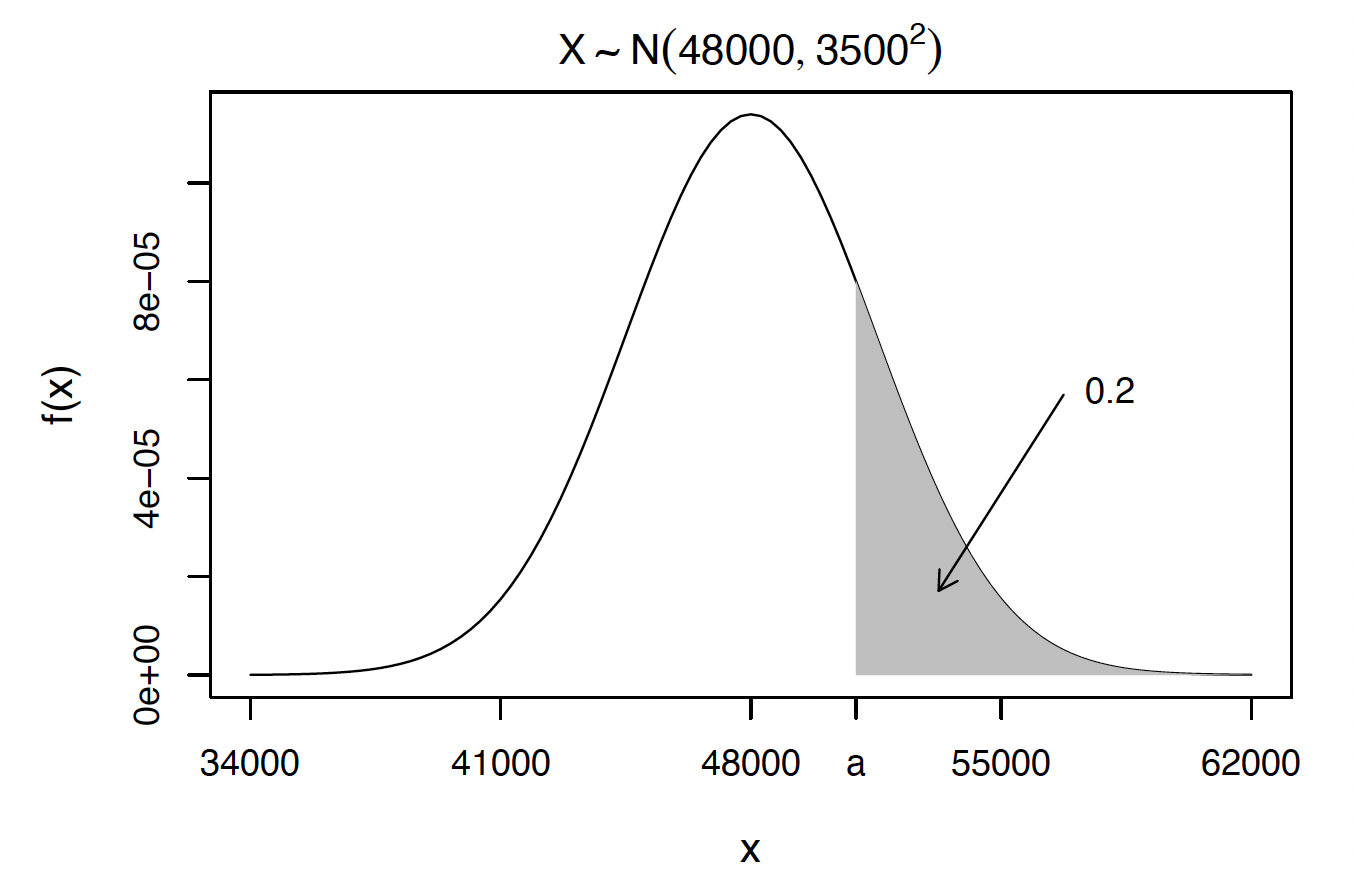
\includegraphics[width=12cm]{example2.png}
\end{frame}

\begin{frame}
	\frametitle{Example 2}
	
	\begin{itemize}
		\item[\color{blue}$\blacktriangleright$] This example is slightly different from the previous.
		\item[\color{blue}$\blacktriangleright$] This time, we essentially have to work \textit{backwards}.
		\item[\color{blue}$\blacktriangleright$] That is, we need to:
		\begin{itemize}
			\item[\color{blue}$\blacktriangleright$] Start with the probability (i.e., 0.2).
			\item[\color{blue}$\blacktriangleright$] Find the $Z$-value that cuts off this probability in the 
			upper tail of the standard normal distribution.
			\item[\color{blue}$\blacktriangleright$] De-standardize this $Z$-value to arrive at the 
			corresponding $X$-value (i.e., $a$), in dollars.
		\end{itemize}
	\end{itemize}
	
\end{frame}
	\begin{frame}
	\frametitle{Example 2: After Standardization}
	\centering
	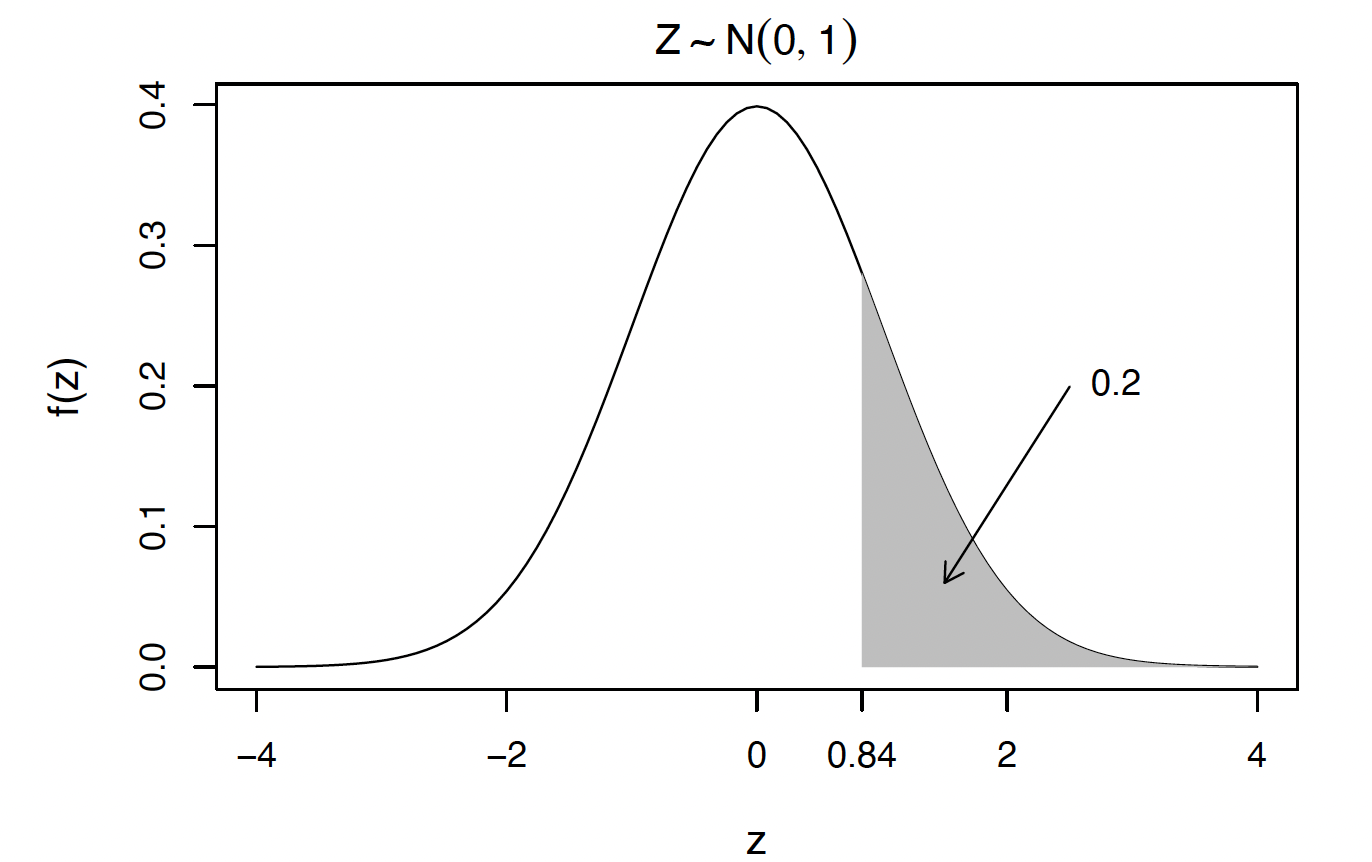
\includegraphics[width=12cm]{example22.png}
\end{frame}
	\begin{frame}
	\frametitle{Example 2}
	\begin{itemize}
		\item[\color{blue}$\blacktriangleright$] $P(Z>z)=0.2$ is the same as $P(Z<z)=0.8$.
	\end{itemize}
	\centering
	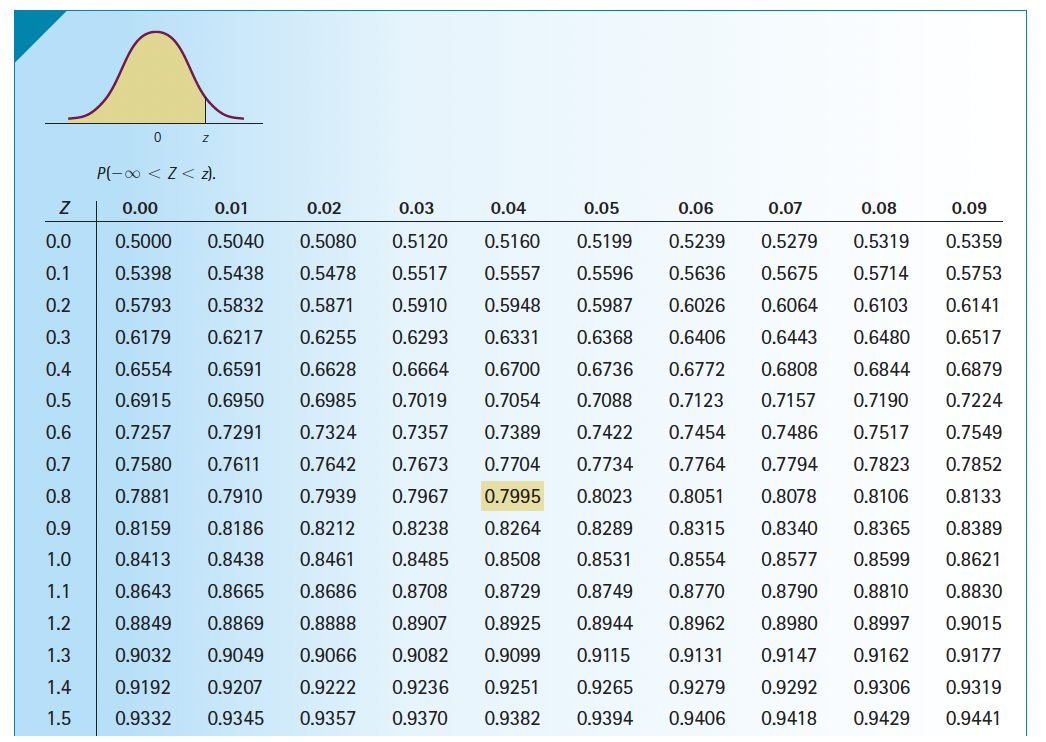
\includegraphics[width=10cm]{example2ztable.png}
\end{frame}

\begin{frame}
	\frametitle{Example 2}
	
	\begin{itemize}
		\item[\color{blue}$\blacktriangleright$] We now have to de-standardize $Z = 0.84$ to find the 
		corresponding value in the $X$-distribution, which is 
		$N(48000, 3500^2)$.
		
		\vspace{0.5em}
		\[
		Z = \frac{X - \mu}{\sigma}
		\]
		\[
		\Rightarrow 0.84 = \frac{X - 48000}{3500}
		\]
		\vspace{0.5em}
		
		\item[\color{blue}$\blacktriangleright$] Solving this for $X$ we get $X = 50940$.
		
		\item[\color{blue}$\blacktriangleright$] Therefore, the minimum salary for the top 20\% of 
		workers is \$50,940.
	\end{itemize}
	
\end{frame}
\begin{frame}
	\frametitle{Example 3}
	
	\begin{itemize}
		\item[\color{blue}$\blacktriangleright$] A soft drink machine can be regulated so that it 
		pours an average of $\mu$ml per cup.
		
		\item[\color{blue}$\blacktriangleright$] If the amount it pours is normally distributed with 
		standard deviation 0.3ml, give the setting for $\mu$ so 
		that 8ml cups will overflow only 1\% of the time.
		
		\item[\color{blue}$\blacktriangleright$] Let $X$ be the amount that the machine pours.
		
		\item[\color{blue}$\blacktriangleright$] Then $X \sim N(\mu, 0.3^2)$.
		
		\item[\color{blue}$\blacktriangleright$] We want to find $\mu$ which makes 8ml cups overflow 
		only 1\% of the time.
	\end{itemize}
	
	\end{frame}
	\begin{frame}
		\frametitle{Example 3}
		
		\begin{itemize}
			\item[\color{blue}$\blacktriangleright$] So we want:
			\[
			P(X > 8) = 0.01
			\]
			
			\item[\color{blue}$\blacktriangleright$] From this probability, we can work backwards to 
			find the corresponding $Z$-value.
			
			\item[\color{blue}$\blacktriangleright$] That is, find $z$ such that $P(Z > z) = 0.01$, or in 
			other words, $P(Z < z) = 0.99$.
			
			\item[\color{blue}$\blacktriangleright$] From the $z$-tables, we get $z = 2.33$.
		\end{itemize}
		
		\end{frame}
		\begin{frame}
			\frametitle{Example 3}
			
			\begin{itemize}
				\item[\color{blue}$\blacktriangleright$] Therefore, if we standardize $X = 8$, we should get 
				$Z = 2.33$:
				
				\vspace{0.5em}
				\[
				Z = \frac{X - \mu}{\sigma}
				\]
				\[
				\Rightarrow 2.33 = \frac{8 - \mu}{0.3}
				\]
				\vspace{0.5em}
				
				\item[\color{blue}$\blacktriangleright$] Solving this for $\mu$ we get $\mu = 7.301$.
				
				\item[\color{blue}$\blacktriangleright$] So the setting for $\mu$ which results in 8ml cups 
				overflowing only 1\% of the time is $\mu = 7.301$.
			\end{itemize}
			
		\end{frame}
\end{document}